\documentclass[a4paper,12pt,notitlepage]{article}
\usepackage{CJKutf8}
\usepackage{indentfirst}
\usepackage{amsmath}
\usepackage{listings}
\usepackage{graphicx}

\begin{CJK*}{UTF8}{gbsn}
\begin{document}

\title{进程间的通信方式}
\author{秦光辉\ 1500011398}
\maketitle

\section{管道通信机制}

	原理:一个进程发出某种数据信息,另一方通过一片共享的存储空间接受数据信息. \\
	
	管道:连接两个进程之间的一个打开的共享文件,用于进程之间的数据通信.类似文件,使用文件读写的方式进行访问,但不是文件,文件系统看不到管道的存在,管道可设在内存. \\
	
	管道通信可由OS核心的缓冲区(通常几十KB)来实现,是单向的. \\
	
	管道通信只能在UNIX和类UNIX系统中实现.简单的管道命令如下:
	
\begin{lstlisting}[frame=shadowbox,numbers=left]
	ls -l | less
\end{lstlisting}

	在这个例子中,ls用于在Unix下列出目录内容,less是一个有搜索功能的交互式的文本分页器.这个管线使得用户可以在列出的目录内容比屏幕长时目录上下翻页. \\
	
	所有广泛应用于UNIX和Windows中的shell程序都有特殊的语法构建管线.典型语法是使用ASCII中的垂直线(正是由于这个原因,这个符号常被称为管道符).当出现这样的语法时shell会启动各个进程,并调整各个进程的标准流之间的连接(还包括安排一些缓存). \\
	
\begin{figure}
\centering
	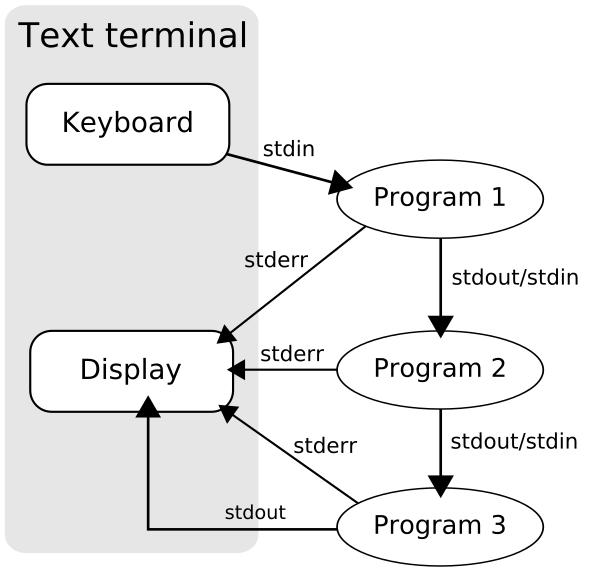
\includegraphics[scale=0.4]{hw4_1.jpeg}
	\caption{文字终端机上一个包含三个程序的管道}
\end{figure}
	
\subsection{UNIX中的匿名管道}

	使用C语言在UNIX中使用pipe(2)系统调用时,这个函数会让系统构建一个匿名管道,这样在进程中就打开了两个新的,打开的文件描述符:一个只读端和一个只写端.管道的两端是两个普通的,匿名的文件描述符,这就让其他进程无法连接该管道. 为了避免死锁并利用进程的并行运行的好处,有一个或多个管道的UNIX进程通常会调用fork(2)产生新进程.并且每个子进程在开始读或写管道之前都会关掉不会用到的管道端.或者进程会产生一个子线程并使用管道来让线程进行数据交换. \\
	
\subsection{UNIX中的具名管道}

	具名管道可以通过调用mkfifo(2)或mknod(2)来构建,当被调用时表现为输入或输出的文件.这样可以允许建立多个管道,并且将其同标准错误重定向或tee结合起来使用更为有效. \\

\section{信号通信机制}

	适用情况:
	
\begin{enumerate}
	\item 想迫使一方对我们的通信立即做出回应
	\item 我们不愿意事先建立任何连接,而是临时突然觉得需要向某个进程通信
	\item 传输信息量微小,使用管道或套接字不划算
\end{enumerate}	

	信号(signal)是一种软中断,传递短消息的简单通信机制,通过发送指定信号来通知进程某个异步事件发生,以迫使进程执行信号处理程序.信号处理完毕后,被中断进程将恢复执行. \\
	
	用户,内核和进程均能生成信号请求.\\
	
\begin{itemize}
	\item 用户:特殊按键
	\item 内核:进程执行出错的时候
	\item 进程:同步信号(进程执行指令而产生的信号),异步信号(像击键之类的进程以外的事件)
\end{itemize}
	
\subsection{Linux实现信号通信的机制}

	Linux信号实现机制包括数据结构,信号的产生和发送,信号的检测和处理. \\
	
\begin{itemize}
	\item 数据结构
	\begin{itemize}
		\item 每个进程task$\_$struct结构中signal域专门保存接收到的信号,内核根据所发生的事件产生相应的信号并发送给接收进程.相当于“中断请求寄存器”的某位置位.
		\item 进程task$\_$struct结构中的blocked是信号屏蔽标记 ,相当于“中断屏蔽寄存器.
		\item 信号处理程序入口 存放在task$\_$struct的sigaction数组中,信号的编号对应于数组下标,数组元素的值是信号处理程序的入口地址.
	\end{itemize}
	\item 信号的产生和发送
	\begin{itemize}
		\item 函数sigaction(signo,act,oldact)信号预置处理程序.
		\item 函数kill(pid,sig)用来向指定进程发送指定信号.
	\end{itemize}
	\item 信号检测和处理流程
	\begin{itemize}
		\item 信号检测与响应发生地点
		\item 信号检测与响应发生时间
		\item 检查处理信号
		\item 信号处理结束
	\end{itemize}
\end{itemize}

\begin{table}
\centering
\begin{tabular}{|c|c|c|}

\hline
Signal & Portable number & Default Action \\
\hline
SIGABRT & 6 & Terminate (core dump) \\
\hline
SIGALRM & 14 & Terminate \\
\hline
SIGBUS & n/a & Terminate (core dump) \\
\hline
SIGCHLD & n/a & Ignore \\
\hline
SIGCONT & n/a & Continue \\
\hline
SIGFPE & n/a & Terminate (core dump) \\
\hline
SIGHUP & 1 & Terminate \\
\hline
SIGILL & n/a & Terminate (core dump) \\
\hline
SIGINT & 2 & Terminate \\
\hline
SIGKILL & 9 & Terminate \\
\hline
SIGPIPE & n/a & Terminate \\
\hline
SIGPOLL & n/a & Terminate \\
\hline
SIGPROF & n/a & Terminate \\
\hline
SIGQUIT & 3 & Terminate (core dump) \\
\hline
SIGSEGV & n/a & Terminate (core dump) \\
\hline
SIGSTOP & n/a & Stop  \\
\hline
SIGSYS & n/a & Terminate (core dump) \\
\hline
SIGTERM & 15 & Terminate \\
\hline
SIGTRAP & n/a & Terminate (core dump) \\
\hline
SIGTSTP & n/a & Stop \\
\hline
SIGTTIN & n/a & Stop \\
\hline
SIGTTOU & n/a & Stop \\
\hline
SIGUSR1 & n/a & Terminate \\
\hline
SIGUSR2 & n/a & Terminate \\
\hline
SIGURG & n/a & Ignore \\
\hline
SIGVTALRM & n/a & Terminate \\
\hline
SIGXCPU & n/a & Terminate (core dump) \\
\hline
SIGXFSZ & n/a & Terminate (core dump) \\
\hline

\end{tabular}
\caption{UNIX中的信号}
\end{table}

\subsection{Windows 信号机制}

	Windows下信号文件$<$signal.h$>$文件的内容如下. \\
	
\begin{lstlisting}[frame=shadowbox,numbers=left,language=C]
// Ctrl-C handler
static int b_ctrl_c = 0;
static int b_exit_on_ctrl_c = 0;

// Signal types
#define SIGINT     2       // interrupt
#define SIGILL     4       // illegal instruction
#define SIGFPE     8       // floating point exception
#define SIGSEGV    11      // segment violation
#define SIGTERM    5       // Software termination
#define SIGBREAK   21      // Ctrl-Break sequence
#define SIGABRT    22      // abnormal termination
\end{lstlisting}
	
	上述向量表中,2表示Ctrl+C中断,4表示非法指令,8表示浮点异常,11表示段错误,5表示Kill发出的软件终止,21表示Ctrl+Break中断,而22是Abort. \\	
	
	Windows下信号处理机制定义在$<$Handler.h$>$中. \\
	
\begin{lstlisting}[frame=shadowbox,numbers=left,language=C]
#include <signal.h>

typedef void (*sighandler_t)(int);
sighandler_t signal(int signum, sighandler_t handler);
\end{lstlisting}
	
\section{信号量通信机制}

	信号量(英语:Semaphore)又称为信号量,旗语,是一个同步对象,用于保持在0至指定最大值之间的一个计数值.当线程完成一次对该semaphore对象等待(wait)时,该计数值减一;当线程完成一次对semaphore对象释放时,计数值加一.当计数值为0,则线程等待该semaphore对象不再能成功直至该semaphore对象变成signaled状态.semaphore对象的计数值大于0,为signaled状态;计数值等于0,为nonsignaled状态.semaphore对象适用于控制一个仅支持有限个用户的共享资源.是一种不需要使用忙碌等待(busy waiting)的一种方法.\\
	
	计数信号量具备两种操作动作,之前称为V(又称signal())与 P(wait()).V操作会增加信号量S的数值,P操作会减少它. \\
	
\subsection{Windows API提供的semphore}

	线程使用CreateSemaphore或CreateSemaphoreEx函数创建一个semaphore对象.此时可以指定semaphore的当前计数值与计数值上限;也可指定semaphore对象的名字.其他进程中的线程可以指出已存在的semaphore对象的名字通过调用OpenSemaphore函数打开它.\\
	
	如果多个线程在等待一个semaphore对象,不保证按照先进先出(FIFO)顺序调度这些等待线程.外部事件,如内核模式的异步过程调用可改变等待顺序.\\

	在semaphore对象为signaled状态时,等待函数返回会把该semaphore对象计数值减1.函数ReleaseSemaphore把semaphore对象的计数值增加指定的值.任何线程,哪怕它没有等待完成过该semaphore对象,也可以使用ReleaseSemaphore来增加semaphore对象的计数.\\

	一个线程多次等待同一个semaphore对象,每次等待操作完成都会降低semaphore对象计数值(直至计数值为0时该线程阻塞).然而,通过multiple-object等待函数使用一个数组包含着同一个semaphore对象的多个句柄,不能实现对这个semaphore对象计数值的多次下降.\\

	用完semaphore对象后,调用CloseHandle函数关闭它.semaphore对象的最后一个句柄被关闭后,操作系统会摧毁它.关闭semaphore并不影响它的计数值.因此,关闭semaphore前或者进程终止前,要确保已经正确调用过ReleaseSemaphore.否则,挂起等待该semaphore对象的线程会永久阻塞或超时返回.\\
	
\subsection{UNXI中的信号量}

	在Unix信号量机制实现之前,通常采用加锁文件的方法.信号量(Semaphore),有时被称为信号灯,是在多线程环境下使用的一种设施,是可以用来保证两个或多个关键代码段不被并发调用.在进入一个关键代码段之前,线程必须获取一个信号量;一旦该关键代码段完成了,那么该线程必须释放信号量.\\

	其它想进入该关键代码段的线程必须等待直到第一个线程释放信号量.为了完成这个过程,需要创建一个信号量VI,然后将Acquire Semaphore VI以及Release Semaphore VI分别放置在每个关键代码段的首末端.确认这些信号量VI引用的是初始创建的信号量.\\

	系统调用semop用来对Unix信号量集合中的一个或多个信号量进行操作,操作命令由用户提供的操作结构数组来定义,该结构如下:

\begin{lstlisting}[frame=shadowbox,numbers=left,language=C]
struct sembuf
{   
	short sem_num;   
	short sem_op;    
	short sem_flg;    
};  
\end{lstlisting}

	系统从用户地址空间读Unix信号量操作结构数组,并核实信号量下标的合法性及进程是否具备读或修改信号量所必需的权限.若权限不够则调用失败;若进程必须睡眠,则它将已操作过的信号量恢复为该系统调用开始时的值,然后它就睡眠,直到它等待的事件发生时再重新执行该系统调用.\\

	由于系统将操作数组保存在一个全局数组中,因此若它必须重新执行该调用的话,它必须重新从用户空间读该数组.这样,操作按原语方式执行--或一次做完或根本不做.\\

	系统根据操作值来改变信号量的值:

\begin{enumerate}
	\item 若操作值为正,系统就增加信号量的值并唤醒所有等待信号量增值的进程;
	\item 若操作值是0,系统就检查信号量的值:如果为0,就继续数组中的其它操作;否则把等待信号量的值为0的睡眠进程数加1,然后睡眠;
	\item 若操作值为负且其绝对值不超过信号量的值,系统就把操作值(一个负数)加到信号量值上,如果结果为0则系统就唤醒所有等待信号量的值为0的睡眠进程;
	\item 若信号量的值小于操作值的绝对值,系统就让进程睡眠在"等待信号量增值"这一事件上.
\end{enumerate}

	当进程在Unix信号量操作过程中睡眠时,它睡眠在可中断级上,因此当它接收到软中断信号时就被唤醒了.用户可在操作标志中设置IPC$\_$NOWAIT标志以防止进程睡眠.\\

	如果进程执行了一个信号量操作,锁住了某些资源,却没有恢复信号量的值就退出了(如收到kill信号),那么就可能出现危险情况.为了避免这类问题,用户可在操作标志中设置SEM$\_$UNDO标志.当进程退出时,系统便撤除该进程做过的每个信号量操作的影响.\\

	值得指出的是,当你使用两个或多个Unix信号量时,死锁总是可能的,系统并不能检查多个信号量间的死锁.\\
	
\section{共享内存}

	共享内存指相互通信的进程间设有公共内存,一组进程向该公共内存中写,另一组进程从公共内存中读,通过这种方式实现两组进程间的信息交换. \\
	
	实现过程如下
	
\begin{enumerate}
	\item 在主存开辟一个公用存储区
	\item 要通信的进程把自己的虚地址空间映射到共享主存区
	\item 发送进程将信息写入共享主存的某个位置时,接收进程可从此位置读取信息
\end{enumerate}

	这是进程通信中最快捷有效的办法.但是需要解决以下问题:
	
\begin{itemize}
	\item 怎样提供共享内存--操作系统提供
	\item 公共内存中的读写互斥问题--程序开发人员负责
\end{itemize}

\subsection{Linx中共享内存的实现方案}

	与信号量一样,在Linux中也提供了一组函数接口用于使用共享内存,而且使用共享共存的接口还与信号量的非常相似,而且比使用信号量的接口来得简单.它们声明在头文件$<$sys/shm.h$>$中.\\

\subsubsection{shmget函数}

	该函数用来创建共享内存,它的原型为:
	
\begin{lstlisting}[frame=shadowbox,numbers=left,language=C]
int shmget(key_t key, size_t size, int shmflg);
\end{lstlisting}

	与信号量的semget函数一样,程序需要提供一个参数key(非0整数),它有效地为共享内存段命名,shmget函数成功时返回一个与key相关的共享内存标识符(非负整数),用于后续的共享内存函数.调用失败返回-1. \\

	不相关的进程可以通过该函数的返回值访问同一共享内存,它代表程序可能要使用的某个资源,程序对所有共享内存的访问都是间接的,程序先通过调用shmget函数并提供一个键,再由系统生成一个相应的共享内存标识符(shmget函数的返回值),只有shmget函数才直接使用信号量键,所有其他的信号量函数使用由semget函数返回的信号量标识符.\\

	第二个参数,size以字节为单位指定需要共享的内存容量. \\

	第三个参数,shmflg是权限标志,它的作用与open函数的mode参数一样,如果要想在key标识的共享内存不存在时,创建它的话,可以与IPC$\_$CREAT做或操作.共享内存的权限标志与文件的读写权限一样,举例来说,0644,它表示允许一个进程创建的共享内存被内存创建者所拥有的进程向共享内存读取和写入数据,同时其他用户创建的进程只能读取共享内存.\\

\subsubsection{shmat函数}

	第一次创建完共享内存时,它还不能被任何进程访问,shmat函数的作用就是用来启动对该共享内存的访问,并把共享内存连接到当前进程的地址空间.它的原型如下:
	
\begin{lstlisting}[frame=shadowbox,numbers=left,language=C]
void *shmat(int shm_id, const void 
*shm_addr, int shmflg);
\end{lstlisting}

	第一个参数,shm$\_$id是由shmget函数返回的共享内存标识.\\
	
	第二个参数,shm$\_$addr指定共享内存连接到当前进程中的地址位置,通常为空,表示让系统来选择共享内存的地址.\\
	
	第三个参数,shm$\_$flg是一组标志位,通常为0.\\

	调用成功时返回一个指向共享内存第一个字节的指针,如果调用失败返回-1. \\
	
\subsubsection{shmdt函数}

	该函数用于将共享内存从当前进程中分离.注意,将共享内存分离并不是删除它,只是使该共享内存对当前进程不再可用.它的原型如下:
	
\begin{lstlisting}[frame=shadowbox,numbers=left,language=C]
int shmdt(const void *shmaddr);
\end{lstlisting}

	参数shmaddr是shmat函数返回的地址指针,调用成功时返回0,失败时返回-1. \\
	
\subsubsection{shmctl函数}

	与信号量的semctl函数一样,用来控制共享内存,它的原型如下:
	
\begin{lstlisting}[frame=shadowbox,numbers=left,language=C]
int shmctl(int shm_id, int command, struct shmid_ds *buf);
\end{lstlisting}
	
	shm$\_$id是shmget函数返回的共享内存标识符.\\
	
	第二个参数,command是要采取的操作,它可以取下面的三个值:
	
\begin{itemize}
	\item IPC$\_$STAT:把shmid$\_$ds结构中的数据设置为共享内存的当前关联值,即用共享内存的当前关联值覆盖shmid$\_$ds的值.
	\item IPC$\_$SET:如果进程有足够的权限,就把共享内存的当前关联值设置为shmid$\_$ds结构中给出的值
	\item IPC$\_$RMID:删除共享内存段
\end{itemize}

	第三个参数,buf是一个结构指针,它指向共享内存模式和访问权限的结构.\\
	
	shmid$\_$ds结构至少包括以下成员:
	
\begin{lstlisting}[frame=shadowbox,numbers=left,language=C]
struct shmid_ds  
{  
	uid_t shm_perm.uid;  
		uid_t shm_perm.gid;  
		mode_t shm_perm.mode;  
};  
\end{lstlisting}

\subsection{Windows下的共享内存}

	Windows下使用共享内存的方式如下:

\subsubsection{设定一块共享内存区域}
     
\begin{lstlisting}[frame=shadowbox,numbers=left,language=C]
HANDLE CreateFileMapping(HANDLE,LPSECURITY_ATTRIBUTES,
 DWORD, DWORD, DWORD,  LPCSTR){
	LPVOID MapViewOfFile(

	HANDLE hFileMappingObject,

	DWORD  dwDesiredAcess,

	DWORD  dwFileOffsetHigh,

	DWORD  dwFileOffsetLow,

	DWORD  dwNumberOfBytesToMap
	);
}
\end{lstlisting}

	得到共享内存的指针. \\
	
\subsubsection{找出共享内存}

	决定这块内存要以点对点(peer to peer)的形式呈现. \\

	每个进程都必须有相同的能力,产生共享内存并将它初始化.每个进程都应该调用CreateFileMapping(),然后调用GetLastError().如果传回的错误代码是ERROR$\_$ALREADY$\_$EXISTS,那么进程就可以假设这一共享内存区域已经被别的进程打开并初始化了,否则该进程就可以合理的认为自己排在第一位,并接下来将共享内存初始化.\\

    只有server进程才应该产生并初始化共享内存.所有的进程都应该使用
    
\begin{lstlisting}[frame=shadowbox,numbers=left,language=C]
HANDLE OpenFileMapping(DWORD dwDesiredAccess, 
BOOL bInheritHandle, LPCTSTR lpName);
\end{lstlisting}

	再调用MapViewOfFile(),取得共享内存的指针. \\
	
\subsubsection{同步处理(Mutex)}

\subsubsection{清理(Cleaning up)}

\begin{lstlisting}[frame=shadowbox,numbers=left,language=C]
BOOL UnmapViewOfFile(LPCVOID lpBaseAddress);
CloseHandle()
\end{lstlisting}

\section{消息传递机制}

	在计算机科学中,消息队列(英语:Message queue)是一种进程间通信或同一进程的不同线程间的通信方式,软件的贮列用来处理一系列的输入,通常是来自用户.消息队列提供了异步的通信协议,每一个贮列中的纪录包含详细说明的数据,包含发生的时间,输入设备的种类,以及特定的输入参数,也就是说:消息的发送者和接收者不需要同时与消息队列互交.消息会保存在队列中,直到接收者取回它.\\

	一个 WIMP 环境像是 Microsoft Windows,借由优先的某些形式(通常是事件的时间或是重要性的顺序)来存储用户产生的事件到一个事件贮列中.系统把每个事件从事件贮列中传递给目标的应用程序.\\

	实际上,消息队列常常保存在链表结构中.拥有权限的进程可以向消息队列中写入或读取消息.\\
	
\subsection{Windows下的消息传递机制}

	在WNDOWS里面消息是很重要的,是WINDOWS的驱动机制,在UNIX当中也含有消息机构,即消息队列,通常用一个消息队列号(KEY,类似于文件描述符来标识文件)标识,通过把一个进程的消息发送进消息队列,其他进程从这个消息队列取消息的方法实现进程通信.消息包含类型,数据长度,数据内容属性,类型和数据长度位于消息首部中,在消息首部中,有指向数据区的指针以及消息队列的链接指针等.\\

	消息机制过程: 

\begin{enumerate}
	\item 首先创建消息队列,系统调用过程中,内核将搜索消息队列头标数组,确定是否存在指定关键字的消息队列.若无,内核将分配一新的队列结构,并返回给用户一个消息队列描述符,如果有,检查消息队列是否可以有访问权限便返回;
	\item 然后使用系统调用发送消息,多个进程间可以把消息放进在同一队列,让同一进程去接收,这样就可以实现多路复用,进入的消息将排在消息队列的尾部;
	\item 接收消息的进程从消息队列中接收消息,如果所返回的消息的大小等于或小于用户请求,内核会将消息拷贝到缓冲区供用户使用,然后消息将被删除,睡眠的发送进程被唤醒.否则返回错误
\end{enumerate} 

	简单代码实现: \\

\begin{lstlisting}[frame=shadowbox,numbers=left,language=C]
int InitQueue(  long* Q_MsgQueue, key_t Q_MsgKey)
{
	*Q_MsgQueue = msgget( (key_t)Q_MsgKey,
	 IPC_CREAT|0666 );
	if( *Q_MsgQueue < 0 )
	{
		printf( "Create Message Queue
		 ERROR!\n");
		return ( -1 );
	}

	return ( 0 );
}

int PutMsgData( char* szBuf, int iBufLen,  
long Q_MsgSnd, int iMsgType)
{
	MSGQUEUE TmpMsgQueue, MsgQueue;
	int  iRet=-1;

	memset( &TmpMsgQueue, 0x00, sizeof(MSGQUEUE));
	memset( &MsgQueue, 0x00, sizeof(MSGQUEUE) );

	MsgQueue.Mtype = MYTYPES;
	MsgQueue.Stype = iMsgType;
	memcpy( MsgQueue.MsgData, szBuf, iBufLen );

	iRet= msgsnd( Q_MsgSnd, &MsgQueue, 
	sizeof(MSGQUEUE), IPC_NOWAIT );
	if( iRet )
	{
	      return ( -1 );
	}

	return ( 0 );
}

int GetMsgData( char* szBuf, long Q_MsgRcv, 
 int iMsgType)
{
          MSGQUEUE MsgQueue;
          int   iLen=0;

          memset( &MsgQueue, 0x00, sizeof(MSGQUEUE) );
          iLen = msgrcv( Q_MsgRcv, &MsgQueue, 
          sizeof(MSGQUEUE)-4, iMsgType, ~IPC_NOWAIT );
          if( iLen < 4 )
         {
	        printf( "Get Msg Data ERROR!\n" );
	         return ( -1 );
          }

          memcpy( szBuf, MsgQueue.MsgData, iLen );

          return ( iLen );
}
\end{lstlisting}
	
\subsection{UNIX下的消息表示方法}

	一个或多个进程可向消息队列写入消息,而一个或多个进程可从消息队列中读取消息,这种进程间通讯机制通常使用在客户/服务器模型中,客户向服务器发送请求消息,服务器读取消息并执行相应请求.在许多微内核结构的操作系统中,内核和各组件之间的基本通讯方式就是消息队列.例如,在 MINIX 操作系统中,内核、I/O任务、服务器进程和用户进程之间就是通过消息队列实现通讯的.\\

	Linux中的消息可以被描述成在内核地址空间的一个内部链表,每一个消息队列由一个IPC的标识号唯一的标识.Linux 为系统中所有的消息队列维护一个 msgque 链表,该链表中的每个指针指向一个 msgid$\_$ds 结构,该结构完整描述一个消息队列.\\

\subsubsection{数据结构}

1.消息缓冲区(msgbuf)

我们在这里要介绍的第一个数据结构是msgbuf结构,可以把这个特殊的数据结构看成一个存放消息数据的模板,它在$<$include/linux/msg.h$>$中声明,描述如下:

\begin{lstlisting}[frame=shadowbox,numbers=left,language=C]
struct msgbuf {

    long mtype;

    char mtext[1];   

};
\end{lstlisting}

	注意:对于消息数据元素(mtext),不要受其描述的限制.实际上,这个域(mtext)不仅能保存字符数组,而且能保存任何形式的任何数据.这个域本身是任意的,因为这个结构本身可以由应用程序员重新定义:

\begin{lstlisting}[frame=shadowbox,numbers=left,language=C]
struct my_msgbuf {
	long mtype;        

	long request_id;  

	struct client info;  
};
\end{lstlisting}

	我们看到,消息的类型还是和前面一样,但是结构的剩余部分由两个其它的元素代替,而且有一个是结构.这就是消息队列的优美之处,内核根本不管传送的是什么样的数据,任何信息都可以传送.\\

	但是,消息的长度还是有限制的,在Linux中,给定消息的最大长度在$<$include/linux/msg.h$>$中定义如下:

\begin{lstlisting}[frame=shadowbox,numbers=left,language=C]
#define MSGMAX 8192    /* max size of message (bytes) */
\end{lstlisting}

	消息总的长度不能超过8192字节,包括mtype域,它是4字节长.\\

2.消息结构(msg)

	内核把每一条消息存储在以msg结构为框架的队列中,它在$<$include/ linux/msg.h$>$中定义如下:

\begin{lstlisting}[frame=shadowbox,numbers=left,language=C]
struct msg {

    struct msg *msg_next;   

    long msg_type;          
    
    char *msg_spot; 

    short msg_ts;
};
\end{lstlisting}

	注意:msg$\_$next是指向下一条消息的指针,它们在内核地址空间形成一个单链表.

3.消息队列结构(msgid$\_$ds)

	当在系统中创建每一个消息队列时,内核创建、存储及维护这个结构的一个实例.

\begin{lstlisting}[frame=shadowbox,numbers=left,language=C]
struct msqid_ds {

    struct ipc_perm msg_perm;

    struct msg *msg_first;  

    struct msg *msg_last;    

    time_t msg_stime;        
    
    time_t msg_rtime;         

    time_t msg_ctime; 

    ushort msg_cbytes;  

    ushort msg_qnum;  

    ushort msg_qbytes;   

    ushort msg_lspid; 

    ushort msg_lrpid;  

};
\end{lstlisting}

\subsubsection{系统调用: msgget()}

	为了创建一个新的消息队列,或存取一个已经存在的队列,要使用msgget()系统调用.  
	                                 
\begin{lstlisting}[frame=shadowbox,numbers=left,language=C]
int msgget ( key_t key, int msgflg );                                            
\end{lstlisting}

	返回: 成功,则返回消息队列识别号,失败,则返回-1,semget()中的第一个参数是键, 这个键值要与现有的键值进行比较,现有的键值指在内核中已存在的其它消息队列的键值.对消息队列的打开或存取操作依赖于msgflg参数的取值: \\

\begin{itemize}
	\item IPC$\_$CREAT : 如果这个队列在内核中不存在,则创建它.
	\item IPC$\_$EXCL :当与IPC$\_$CREAT一起使用时,如果这个队列已存在,则创建失败.
\end{itemize}

	如果IPC$\_$CREAT单独使用,semget()为一个新创建的消息队列返回标识号,或者返回具有相同键值的已存在队列的标识号.如果IPC$\_$EXCL与IPC$\_$CREAT一起使用,要么创建一个新的队列,要么对已存在的队列返回-1.IPC$\_$EXCL单独是没有用的,当与IPC$\_$CREAT结合起来使用时,可以保证新创建队列的打开和存取.\\

	与文件系统的存取权限一样,每一个IPC对象也具有存取权限,因此,可以把一个八进制与掩码或,形成对消息队列的存取权限.\\

	让我们来创建一个打开或创建消息队列的函数:

\begin{lstlisting}[frame=shadowbox,numbers=left,language=C]
int open_queue( key_t keyval )

{

        int     qid;

        if((qid = msgget( keyval, IPC_CREAT
         | 0660 )) == -1)

	     return(-1);

        return(qid);

}
\end{lstlisting}

	注意,这个例子显式地用了0660权限.这个函数要么返回一个消息队列的标识号,要么返回-1而出错.键值作为唯一的参数必须传递给它.

\subsection{系统调用: msgsnd()}

	一旦我们有了队列识别号,我们就可以在这个队列上执行操作.要把一条消息传递给一个队列,你必须用msgsnd()系统调用.

\begin{lstlisting}[frame=shadowbox,numbers=left,language=C]
int msgsnd ( int msqid, struct msgbuf *msgp, 
int msgsz, int msgflg );
\end{lstlisting}

	msgsnd()的第一个参数是队列识别号,由msgget()调用返回.第二个参数msgp是一个指针,指向我们重新声明和装载的消息缓冲区.msgsz参数包含了消息以字节为单位的长度,其中包括了消息类型的4个字节.\\

	msgflg参数可以设置成0(忽略),或者: \\

	IPC$\_$NOWAIT :如果消息队列满,消息不写到队列中,并且控制权返回给调用进程(继续执行).如果不指定IPC$\_$NOWAIT,调用进程将挂起(阻塞)直到消息被写到队列中.\\

	让我们来看一个发送消息的简单函数:

\begin{lstlisting}[frame=shadowbox,numbers=left,language=C]
int send_message( int qid, struct mymsgbuf *qbuf )
{

	int result, length;

	length = sizeof(struct ) - sizeof(long);       

	if((result = msgsnd( qid, qbuf, length, 0))
	 == -1)

	return(-1);

	return(result);
}
\end{lstlisting}

	这个小函数试图把缓冲区qbuf中的消息,发送给队列识别号为qid的消息队列.\\

	现在,我们在消息队列里有了一条消息,可以用ipcs命令来看你队列的状态.如何从消息队列检索消息,可以用msgrcv()系统调用.\\

\subsection{系统调用:msgrcv()}                                                 

\begin{lstlisting}[frame=shadowbox,numbers=left,language=C]
int msgrcv ( int msqid, struct msgbuf *msgp,
 int msgsz, long mtype, int msgflg );
\end{lstlisting}

   返回值:成功,则为拷贝到消息缓冲区的字节数,失败为-1.\\

	很明显,第一个参数用来指定要检索的队列(必须由msgget()调用返回),第二个参数(msgp)是存放检索到消息的缓冲区的地址,第三个参数(msgsz)是消息缓冲区的大小,不包括消息类型mtype的长度.\\

	第四个参数(mtype)指定了消息的类型.内核将搜索队列中相匹配类型的最早的消息,并且返回这个消息的一个拷贝,返回的消息放在由msgp参数指向的地址.这里存在一个特殊的情况,如果传递给mytype参数的值为0,就可以不管类型,只返回队列中最早的消息.\\

	如果传递给参数msgflg的值为IPC$\_$NOWAIT,并且没有可取的消息,那么给调用进程返回ENOMSG错误消息,否则,调用进程阻塞,直到一条消息到达队列并且满足msgrcv()的参数.如果一个客户正在等待消息,而队列被删除,则返回EIDRM.如果当进程正在阻塞,并且等待一条消息到达但捕获到了一个信号,则返回EINTR.\\

	让我们来看一个从我们已建的消息队列中检索消息的例子

\begin{lstlisting}[frame=shadowbox,numbers=left,language=C]
int read_message( int qid, long type, 
struct mymsgbuf *qbuf )

{

	int result, length;

	length = sizeof(struct mymsgbuf)
	 - sizeof(long);       

	if((result = msgrcv( qid, qbuf,
	 length, type, 0)) == -1)
		return(-1);

	return(result);

}
\end{lstlisting}

	当从队列中成功地检索到消息后,这个消息将从队列删除.
	
\section{套接字}

	UNIX BSD 首创的网络通信机制,提供进程通信端口,socket是面向客户-服务器模式设计的底层通信机制. \\
	
	套接字是TCP/IP网络通信的基本构件之一,必须有客户端和服务器端两个进程,通过无连接协议或有连接协议服务的调用时序进行工作. \\
	
	使用套接字进行通信的双方均需创建一个套接字,其中一方作为服务器方,另外一方作为客户方. \\
	
\begin{enumerate}
	\item 服务器方先创建一个服务器套接字,然后在该套接字上监听,等待远方的连接请求.
	\item 客户则创建一个客户套接字,向服务区套接字发送连接请求.
	\item 服务器套接字收到连接请求后,将在服务器机器上创建一个客户套接字,与远方客户机上的客户套接字形成点到点的通信.
	\item 客户端与服务器端通过send和recv命令在所创建的套接字上进行交流
\end{enumerate}	
	
\end{CJK*}
\end{document}